\section{SAMCell Data Flow}
\label{sec:samcell-detail}

The diagram in~\Cref{fig:samcell} shows the various modules of 
SAM Cell and describes the flow of information between them.
In the figure, the gray box on the left shows SAM Cell processing the $k$-th frame of the video, whose feature map equals $F_k$, for $T$ reasoning steps.
The contextual words $\vec{cw}$ and question embedding $\vec{q}$ form the remaining
inputs to SAM Cell.
The state of memory (contents) at the beginning of this reasoning process is denoted by $M_0$. This is updated for each of the $T$ reasoning steps along with the various recurrent states of SAM Cell, namely, $\vec{wh}_t$, $\vec{c}_t$ and $\vec{so}_t$. 
The gray box on the right details what happens across the various modules
during a single reasoning step $t$.
The main document describes the role played by each tensor shown going between
various modules within that box.
\begin{figure*}[hbtp]
	\centering
	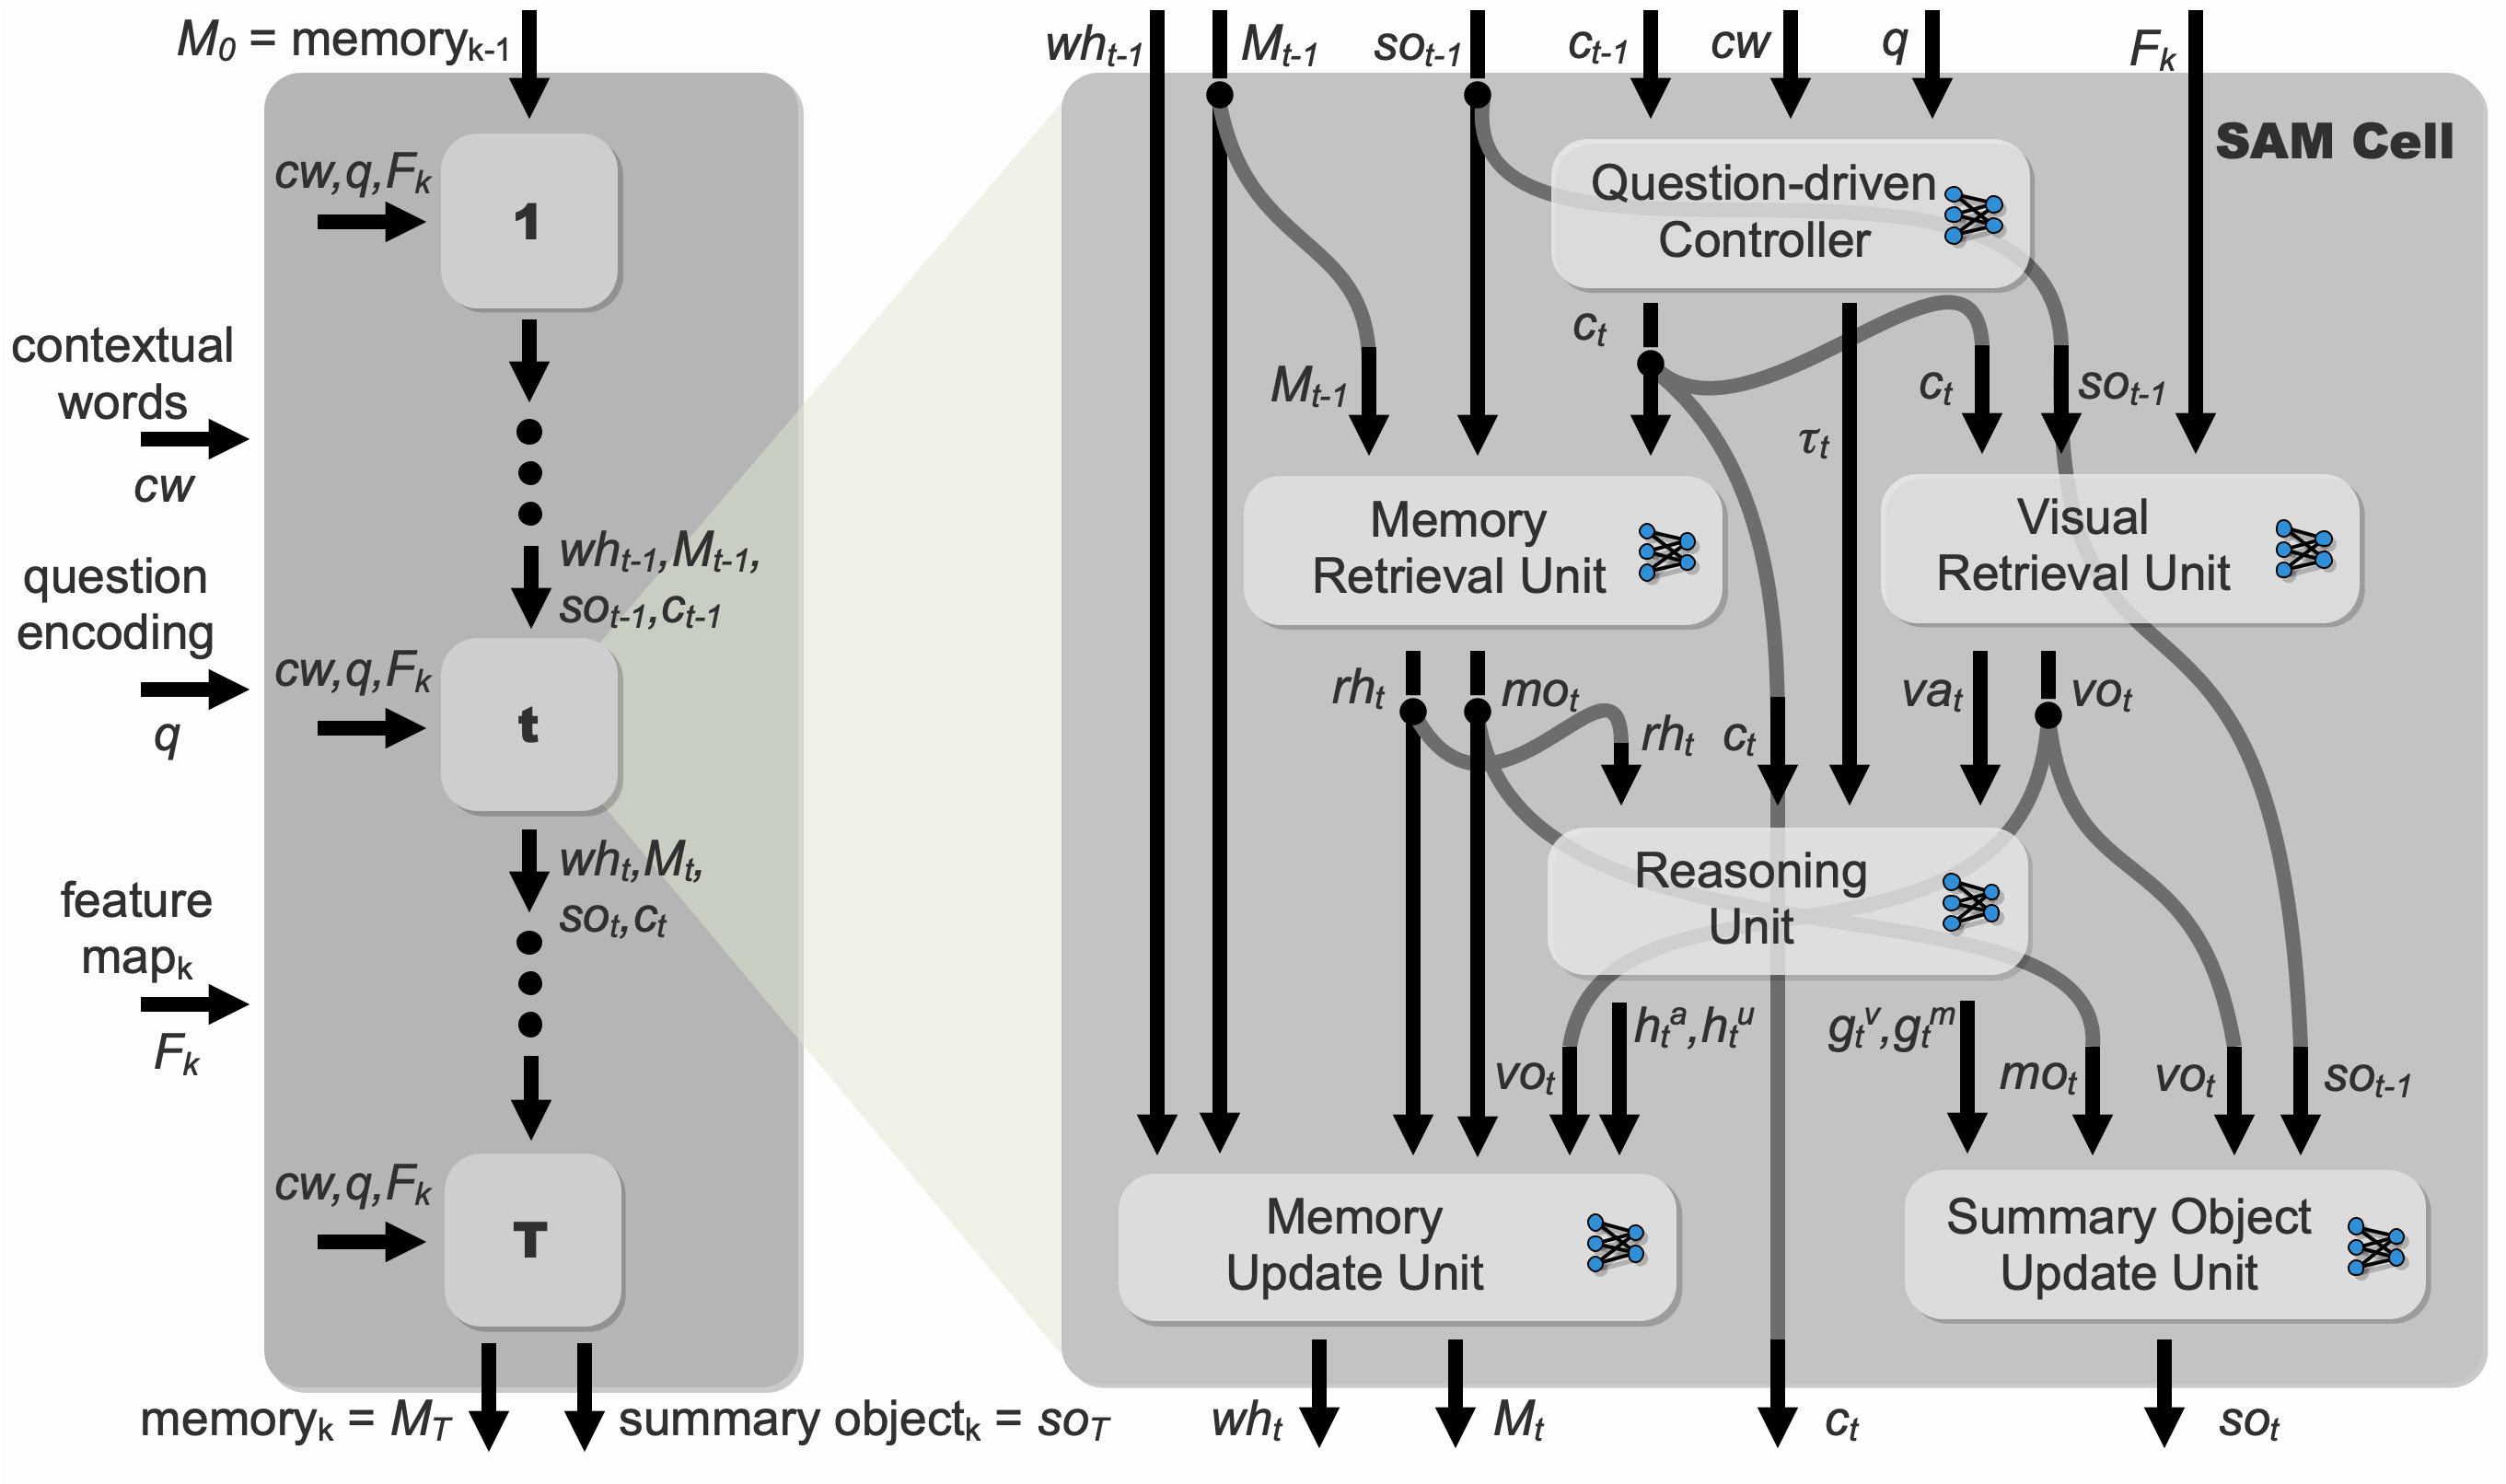
\includegraphics[width=\textwidth]{../img/architecture/samcell_reasoning}
	\caption{Archirecture of SAM Cell.}
	\label{fig:samcell}
\end{figure*}

\clearpage

\section{Datasets: CLEVR-CoGenT and COG}
\label{sec:datasets-desc}
%Here are the details of the COG dataset.
%
The CoGenT dataset~\cite{johnson2017clevr} contains:
\begin{itemize}
	\def\labelitemi{--}
	\item Training set of 70,000 images and 699,960 questions in Condition A,
	\item Validation set of 15,000 images and 149,991 questions in Condition A,
	\item Test set of 15,000 images and 149,980 questions in Condition A (without answers),
	\item Validation set of 15,000 images and 150,000 questions in Condition B,
	\item Test set of 15,000 images and 149,992 questions in Condition B (without answers),
	\item Scene graphs and functional programs for all training / validation images and questions.
\end{itemize}

\noindent The combinations of attributes in CoGenT-A and CoGenT-B are shown in~\cref{tab:cogent_conditions_supplement}.
\begin{table}[ht]
	\centering
	\begin{tabular}{cccc}
		\toprule
		Dataset	&	Cubes	&	Cylinders	&	Spheres	\\
		\midrule
		CoGenT-A	&	Gray / Blue / Brown / Yellow	&	Red / Green / Purple / Cyan	&	Any color	\\
		CoGenT-B	&	Red / Green / Purple / Cyan	&	Gray / Blue / Brown / Yellow	&	Any color 	\\
		\bottomrule
	\end{tabular}
	\smallskip
	\caption{Colors \& shapes combinations present in CoGenT-A \& -B datasets.}
	\label{tab:cogent_conditions_supplement}
\end{table}

\noindent The Canonical and Hard variants of the COG dataset~\cite{yang2018dataset} are contrasted in~\cref{tab:cog_variants_supplement}.
\begin{table}[ht]
	\centering
	\begin{tabular}{lcccccc}
		\toprule
		Variant    &  	number &  	maximum & maximum & size & size & size  \\
		& of   & memory & number of & of & of & of  \\
		& frames & duration & distractors & training set & validation set & test set \\
		\midrule
		Canonical & 4 & 3 & 1 & 10000320 & 500016 & 500016 \\
		Hard  & 8 & 7 & 10 & 10000320 & 500016  & 500016 \\
		\bottomrule
	\end{tabular}
	\smallskip
	\caption{Details of the Canonical and Hard variants of the COG dataset.}
	\label{tab:cog_variants_supplement}
\end{table}
%
%\begin{table}[ht]
%	\centering
%	\begin{tabular}{lcccccc}.
%		\toprule
%		Variant    &  	number &  	maximum & maximum & size & size & size  \\
%		& of   & memory & number of & of & of & of
%%		& frames & duration & distractors & training set & validation set & test set \\
%		\midrule
%		Canonical & 4 & 3 & 1 & 10000320 & 500016 & 500016 \\
%		Hard  & 8 & 7 & 10 & 10000320 & 500016  & 500016 \\
%		\bottomrule
%	\end{tabular}
%	\caption{Details of the Canonical and Hard variants of the COG dataset.}
%	\label{tab:cog_variants_supplement}
%\end{table}



\clearpage
\section{Complete COG results}
\label{sec:cog-all-results}

\begin{table*}[htb]
	\centering
	\begin{adjustbox}{width=\textwidth}
		\begin{tabular}{l r r r r r r r r r r}
			\toprule[1.25pt]
			Model & \multicolumn{4}{c}{SAMNet} &  &\multicolumn{4}{c}{Baseline Model} \\
			\cmidrule(lr){2-5}
			\cmidrule(lr){7-10}
			&&&&& & paper & code & code & paper\\
			\cmidrule(lr){7-10}
			Trained on       & canonical & canonical & canonical & hard &           &  canonical  & canonical  & canonical & hard \\
			Fine tuned on  & - & - & hard  & - &           & -   & - & hard & - \\
			Tested on        & canonical & hard & hard & hard &            &canonical  & hard & hard & hard  \\
			\midrule[1pt]
			Overall accuracy & 98.0 & 91.6 & 96.5  & 96.1 &           & 97.6  & 65.9 & 78.1& 80.1 \\
			\midrule[1pt]
			AndCompareColor			&	93.5	&	82.7	&	89.2	&	80.6	&	&	81.9	&	57.1	&	60.7	&	51.4	 \\
			AndCompareShape			&	93.2	&	83.7	&	89.7	&	80.1	&	&	80.0	&	53.1	&	50.3	&	50.7 \\
			AndSimpleCompareColor		&	99.2	&	85.3	&	97.6	&	99.4	&	&	99.7	&	53.4	&	77.1	&	78.2 \\
			AndSimpleCompareShape		&	99.2	&	85.8	&	97.6	&	99.2	&	&	100.0	&	56.7	&	79.3	&	77.9 \\
			CompareColor			&	98.1	&	89.3	&	95.9	&	99.7	&	&	99.2	&	56.1	&	67.9	&	50.1 \\
			CompareShape			&	98.0	&	89.7	&	95.9	&	99.2	&	&	99.4	&	66.8	&	65.4	&	50.5	 \\
			Exist				&	100.0	&	99.7	&	99.8	&	99.8	&	&	100.0	&	63.5	&	96.1	&	99.3 \\
			ExistColor			&	100.0	&	99.6	&	99.9	&	99.9	&	&	99.0	&	70.9	&	99	&	89.8 \\
			ExistColorOf			&	99.9	&	95.5	&	99.7	&	99.8	&	&	99.7	&	51.5	&	76.1	&	73.1 \\
			ExistColorSpace			&	94.1	&	88.8	&	91.0	&	90.8	&	&	98.9	&	72.8	&	77.3	&	89.2 \\
			ExistLastColorSameShape		&	99.5	&	99.4	&	99.4	&	98.0	&	&	100.0	&	65.0	&	62.5	&	50.4 \\
			ExistLastObjectSameObject	&	97.3	&	97.5	&	97.7	&	97.5	&	&	98.0	&	77.5	&	61.7	&	60.2 \\
			ExistLastShapeSameColor		&	98.2	&	98.5	&	98.8	&	97.5	&	&	100.0	&	87.8	&	60.4	&	50.3 \\
			ExistShape			&	100.0	&	99.5	&	100.0	&	100.0	&	&	100.0	&	77.1	&	98.2	&	92.5 \\
			ExistShapeOf			&	99.4	&	95.9	&	99.2	&	99.2	&	&	100.0	&	52.7	&	74.7	&	72.70 \\
			ExistShapeSpace			&	93.4	&	87.5	&	91.1	&	90.5	&	&	97.7	&	70.0	&	89.8	&	89.80 \\
			ExistSpace			&	95.3	&	89.7	&	93.2	&	93.3	&	&	98.9	&	71.1	&	88.1	&	92.8 \\
			GetColor			&	100.0	&	95.8	&	99.9	&	100.0	&	&	100.0	&	71.4	&	83.1	&	97.9 \\
			GetColorSpace			&	98.0	&	90.0	&	95.0	&	95.4	&	&	98.2	&	71.8	&	73.	&	92.3 \\
			GetShape			&	100.0	&	97.3	&	99.9	&	99.9	&	&	100.0	&	83.5	&	89.2	&	97.1	 \\
			GetShapeSpace			&	97.5	&	89.4	&	93.9	&	94.3	&	&	98.1	&	78.7	&	77.3	&	90.3 \\
			SimpleCompareShape		&	99.9	&	91.4	&	99.7	&	99.9	&	&	100.0	&	67.7	&	96.7	&	99.3 \\
			SimpleCompareColor		&	100.0	&	91.6	&	99.80	&	99.9	&	&	100.0	&	64.2	&	90.4	&	99.3 \\
			\bottomrule[1.25pt]
		\end{tabular}
	\end{adjustbox}
	\smallskip
	\caption{COG test set accuracies for SAMNet and the baseline model~\cite{yang2018dataset}. For the baseline model,
		`paper' denotes results reproduced from~\cite{yang2018dataset} along with some further clarifications by the authors (private communication)  regarding the performance on individual task types while `code' denotes results of our experiments using their implementation~\cite{yang2018implement}.}
	\label{tab:all-results}
\end{table*}

\clearpage
\section{Complete CLEVR-CoGenT results}
\label{sec:full-cogent-results}

\begin{table*}[htb]
	\centering
	\begin{adjustbox}{width=\textwidth}
	\begin{tabular}{c c c c c c c }\toprule
		\multicolumn{1}{c }{\textbf{}} & \multicolumn{6}{c }{\textbf{Test Accuracy (\%)}} \\
		\multicolumn{1}{c }{\textbf{}} & \multicolumn{6}{c }{on \texttt{valA} -- 150,000 samples} \\
		\cmidrule(lr){2-7}
		\multicolumn{1}{ c }{\textbf{Experiments}} & \textbf{Overall}& \textbf{Exist}  & \textbf{Count} & \textbf{CompareInteger} & \textbf{CompareAttribute} & \textbf{QueryAttribute}\\
		\cmidrule(lr){1-1}
		\cmidrule(lr){2-7}
		\multicolumn{1}{ c }{Exist only} & 26.07 & \emph{74.20}	& 0.0	& 59.79	& 59.15 & 0.0 \\
		\multicolumn{1}{ c }{Count only} & 14.89  & 0.0	& \emph{62.78}	& 0.0 & 0.0 & 0.0 \\
		\multicolumn{1}{ c }{CompareInteger only} & 23.44 & 48.15	& 0.0	& \emph{77.98}	& 54.08 & 0.0 \\
		\multicolumn{1}{ c }{CompareAttribute only} & 23.50 & 51.93	& 0.0 & 59.06 & \emph{61.73} & 0.0 \\
		\multicolumn{1}{ c }{QueryAttribute only} & 34.64 	& 0.0	& 0.0	& 0.0 & 0.0 & \emph{97.08} \\
		\cmidrule(lr){1-1}
		\cmidrule(lr){2-7}

		\multicolumn{1}{ c }{All tasks} & 95.32 & 98.4 	& 86.75	& 96.0	& 98.65	& 98.02 \\
		\cmidrule(lr){1-1}
		\cmidrule(lr){2-7}

		\multicolumn{1}{ c }{All tasks but Exist} & 90.33 	& \emph{60.42}	& 86.12	& 96.18	& 98.52 & 98.60 \\
		\multicolumn{1}{ c }{All tasks but Count} & 74.59 	& 97.51	& \emph{0.0}	& 94.37	& 98.42 & 98.47 \\
		\multicolumn{1}{ c }{All tasks but CompareInteger} & 91.53 	& 98.22	& 86.09	& \emph{56.35}	& 98.78 & 98.40 \\
		\multicolumn{1}{ c }{All tasks but CompareAttribute} & 81.92 	& 98.32	& 86.36	& 95.86	& \emph{23.18} & 98.44 \\
		\multicolumn{1}{ c }{All tasks but QueryAttribute} & 42.17 	& 76.79	& 54.64	& 79.87 & 64.13 & \emph{0.0} \\

		\cmidrule(lr){1-1}
		\cmidrule(lr){2-7}

		\multicolumn{1}{ c }{\textit{Trained on all tasks -- Finetune on $t$}} & &  & &  & &\\
		\multicolumn{1}{ c }{Exist} & 94.16 & \emph{98.04} & 82.96 & 95.02 & 98.12 & 97.97 \\
		\multicolumn{1}{ c }{Count} & 95.10 & 96.46 & \emph{88.28} & 94.78 & 97.01 & 98.26 \\
		\multicolumn{1}{ c }{CompareInteger} & 95.31 & 98.39 & 86.56 & \emph{96.07} & 98.70 & 98.09 \\
		\multicolumn{1}{ c }{CompareAttribute} & 95.31 & 98.40 & 86.78 & 96.00 & \emph{98.66} & 98.04 \\
		\multicolumn{1}{ c }{QueryAttribute} & 93.49 & 97.45 & 82.09 & 92.23 & 97.85& \emph{97.76} \\

		\bottomrule
	\end{tabular}
	\end{adjustbox}
    \smallskip
	\caption{Complete set of results for SAMNet on CLEVR-CoGenT.}
	\label{tab:CoGenT-results}
\end{table*}
